\subsection{Simulation-Based Jet Background Cuts and Efficiencies}
\label{sec:sim_jet_background}

Jet background rejection cuts are first studied in simulation to assess their impact on the underlying event (UE) measurement. 
Two primary background rejection strategies are considered: calorimeter layer energy fraction cut and a dijet topology cut.

Figures~\ref{fig:sim_efrac_bkg_tr_et} and~\ref{fig:sim_dijet_bkg_tr_et} show the impact of the energy fraction cut and dijet cut respectively on the transverse region $E_{T}$ distribution. 
The energy fraction cut does not bias the reconstructed UE measurement, while the dijet cut introduces a small bias at the 5--10\% level.
Therefore, the energy fraction cut is used as the primary simulation-driven jet background cut, and additional data-driven timing cuts are developed and are also applied to the data to remove additional jet backgrounds not accounted for in the energy fraction cut.
Figure~\ref{fig:sim_efrac_bkg_jetpt} shows the effect of the energy fraction cut on the reconstructed jet $p_{T}$ distribution in the analysis measurement range.
\begin{figure}
    \centering
    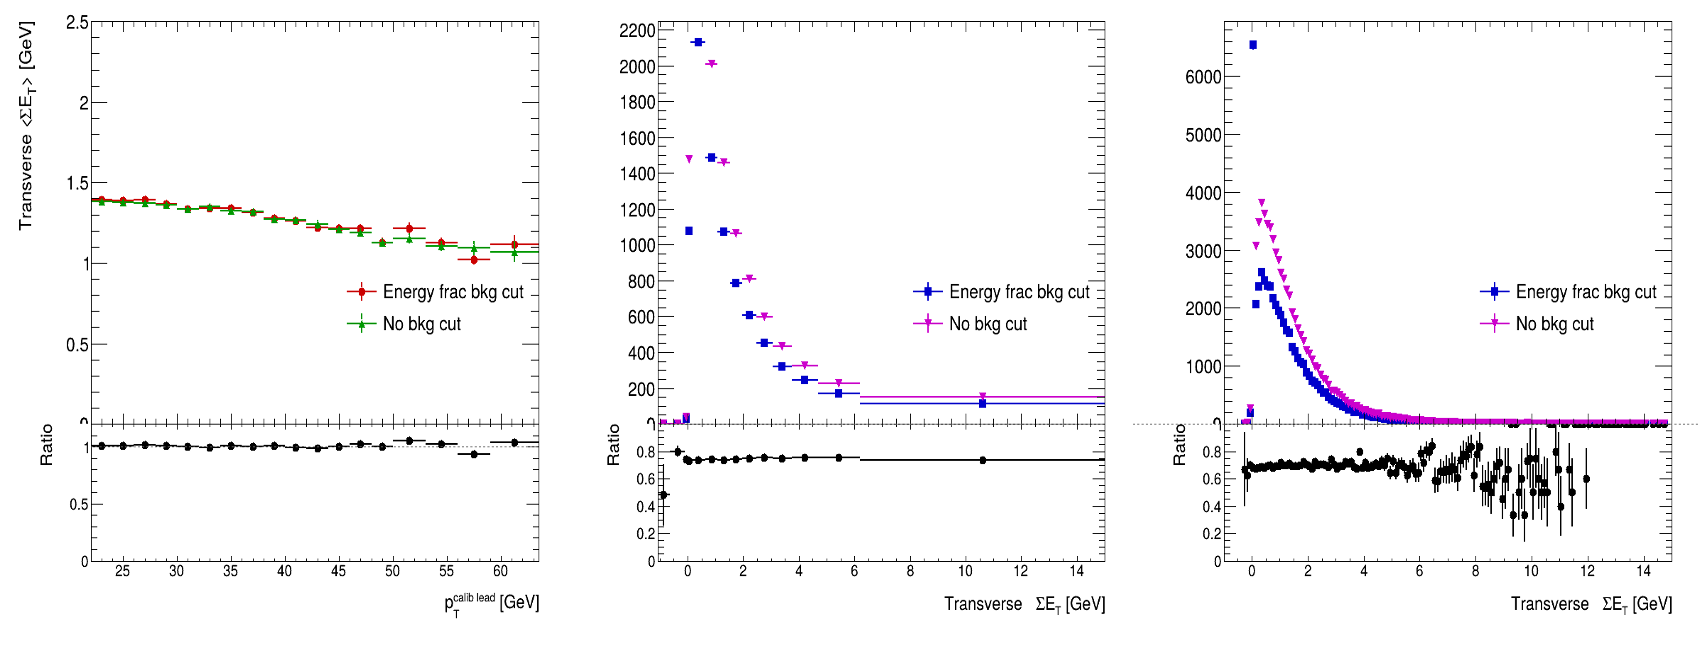
\includegraphics[width=\linewidth]{Figures/jet_bkg_cuts/sim_based_efrac_bkg_cuts.png}
    \caption{Effect of the energy fraction cut on the transverse region $E_{T}$ distribution in the analysis measurement range. The left plot shows the bias on the reco level $\langle \Sigma E_{T} \rangle$ as a function of calibrated reco leading jet $p_{T}$, the middle plot shows the efficiency of the energy fraction background cut on the reco level transverse region $E_{T}$ distribution with binning used in analysis, the right plot shows the efficiency of the energy fraction background cut on the reco level transverse region $E_{T}$ distribution with finer binning to test any binning effects.}
    \label{fig:sim_efrac_bkg_tr_et}
\end{figure}
\begin{figure}
    \centering
    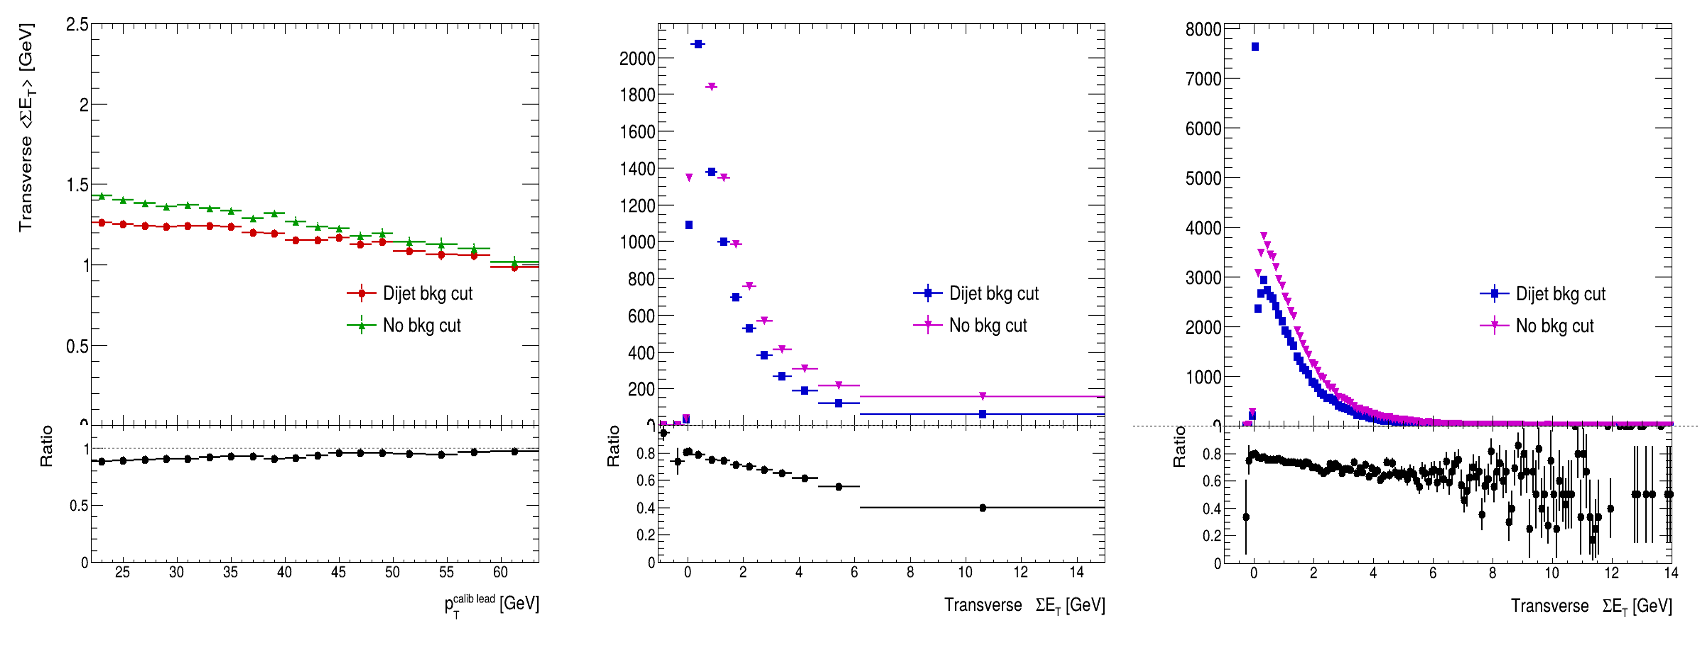
\includegraphics[width=\linewidth]{Figures/jet_bkg_cuts/sim_based_dijet_bkg_cuts.png}
    \caption{Effect of the dijet cut on the transverse region $E_{T}$ distribution in the analysis measurement range. The left plot shows the bias on the reco level $\langle \Sigma E_{T} \rangle$ as a function of calibrated reco leading jet $p_{T}$, the middle plot shows the efficiency of the dijet background cut on the reco level transverse region $E_{T}$ distribution with binning used in analysis, the right plot shows the efficiency of the energy fraction background cut on the reco level transverse region $E_{T}$ distribution with finer binning to test any binning effects.}
    \label{fig:sim_dijet_bkg_tr_et}
\end{figure}
\begin{figure}
    \centering
    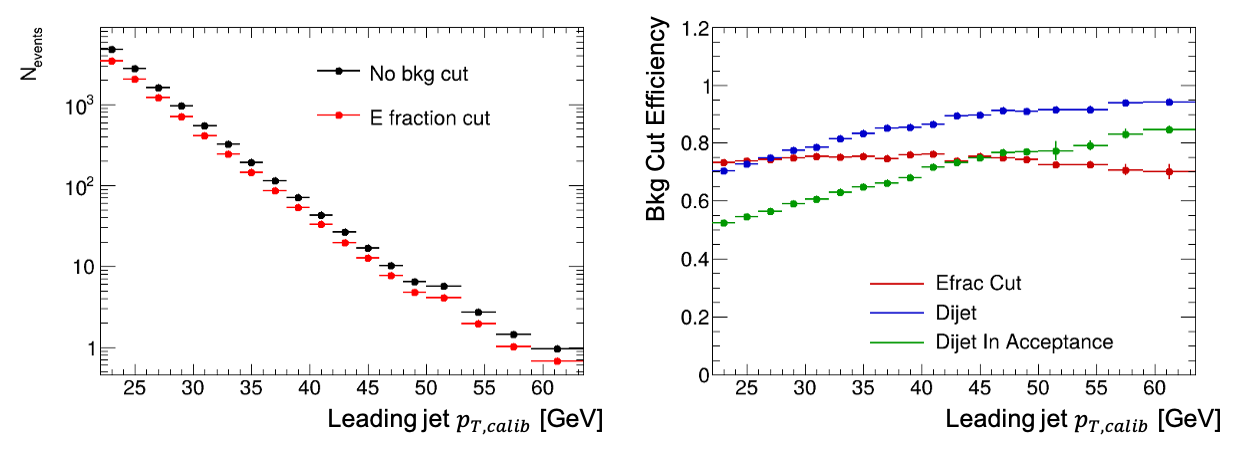
\includegraphics[width=\linewidth]{Figures/jet_bkg_cuts/sim_based_efrac_bkg_cuts_jet_effects.png}
    \caption{Effect of the energy fraction cut on the reconstructed leading jet $p_{T}$ distribution for inclusive jets in the analysis measurement range. (Left) Leading jet yield for inclusive jet events with and without the energy fraction cut. (Right) Efficiency of background cut application on jet yield in inclusive jet events for a variety of jet background cuts (only energy fraction cut used in inclusive jet analysis).} 
    \label{fig:sim_efrac_bkg_jetpt}
\end{figure}

\subsection{Data-Driven Jet Background Timing Cuts}
\label{sec:data_jet_timing}

Additional jet background rejection cuts are applied to both the inclusive jet and dijet samples to remove additional jet backgrounds not accounted for in the energy fraction cut and dijet cut, respectively.
For the dijet sample, the additional data-driven jet background cuts used are cuts on the leading jet time and time difference between the leading and subleading jet developed by JSTG TF1~\cite{tf1_note} and implemented in PPG08/PPG09 \cite{ppg08AN,ppg09AN}. For the inclusive jet sample, the sample leading time cut from JSTG TF1~\cite{tf1_note} is applied and an additional data-driven jet background rejection cut is developed and implemented for this inclusive jet sample by using the timing correlation between the leading jet and the MBD since a subleading jet may not be available in the inclusive jet case. Table~\ref{tab:jet_background_cuts} outlines the full set of jet background cuts applied to the inclusive jet and dijet analyses respectively.

\begin{table}[]
    \centering
    \begin{tabular}{c|c}
        \multicolumn{2}{c}{Inclusive Jet Events} \\
        \hline
        Cut Name & Application \\
        \hline
        E fraction cut & EMCal(10-90\%)/IHCal(0-90\%)/OHCal(10-90\%) E frac on lead jet \\
        Leading jet time cut & Require lead jet time in $[-8,4]$ ns \\
        Lead jet--MBD time diff cut & Require lead jet--MBD $\Delta t$ in $[-5,1]$ ns \\
    \end{tabular} \\
    \bigskip \bigskip
    \begin{tabular}{c|c}
        \multicolumn{2}{c}{Dijet Events} \\
        \hline
        Cut Name & Application \\
        \hline
        Dijet cut & Require $E_{\mathrm{sub}}/E_{\mathrm{lead}}>0.3$, $\Delta\phi>\Delta\phi_{\mathrm{min}} = 3\pi / 4$ \\
        Leading jet time cut & Require lead jet time in $[-8,4]$ ns \\
        Lead--sublead jet time diff cut & Require lead--sublead jet $\Delta t$ in $[-3,3]$ ns \\
    \end{tabular}
    \caption{Outline of jet background cuts applied to inclusive jet (top) and dijet (bottom) samples respectively.}
    \label{tab:jet_background_cuts}
\end{table}

Detailed information on the development and investigation of this additional jet--MBD time difference cut are included in Appendix~\ref{sec:jet_mbd_time_bkg_cut} while an example of the jet--MBD time difference distribution with cut bounds shown as well as the cut's efficiency and purity determination are included below. The same methodology and same fitting code as in JSTG TF1~\cite{tf1_note} was used to determine the timing cut efficiency and purity for this jet--MBD time cut.
Specifically, the cut efficiency and purity are extracted by fitting the leading jet time and jet--MBD time distributions with a Gaussian plus constant background fit. 
A leading jet timing window of $[-8,4]$~ns is used for the signal region same as is done in PPG09. 
Based on the jet--MBD time difference distribution, a $\Delta t_{\mathrm{jet-MBD}}$ requirement of $[-5,1]$~ns is selected. 
The positive tail beyond 0~ns is attributed primarily to pileup.
The extracted signal and signal + background distributions are shown in Figure~\ref{fig:lead_jet_time_mbd_time_cut}.

Timing cut efficiencies are extracted using the same fitting methodology employed in JSTG TF1, with the only difference being using the jet--MBD time instead of the dijet time difference.
The extracted efficiencies as a function of leading jet $p_{T}$ are shown in Figure~\ref{fig:timing_cut_efficiencies}.
The jet timing cut efficiencies are around 98\% for the nominal leading jet time and jet--MBD time cuts and above 99\% for the variations of the nominal cuts which widen the timing windows by 1~ns.
Similar efficiency values are observed ($>\sim$95\%) for the leading jet time + dijet time difference cuts in JSTG TF1.

These timing cuts are applied in data at the reconstruction level to remove additional jet backgrounds not accounted for in the energy fraction and dijet cuts.
The timing cut efficiencies are also applied at the reconstruction level to data events, the reconstructed data with both these nominal and variation efficiency values applied are propagated through the analysis chain and unfolding procedure.
The purity of the timing cuts is also extracted and shown in Figure~\ref{fig:timing_cut_purity}.
The timing cuts have a very high purtiy ($>$99\%) for all but the last leading jet $p_{T}$ bin where the results are statistics limited.

\begin{figure}
    \centering
    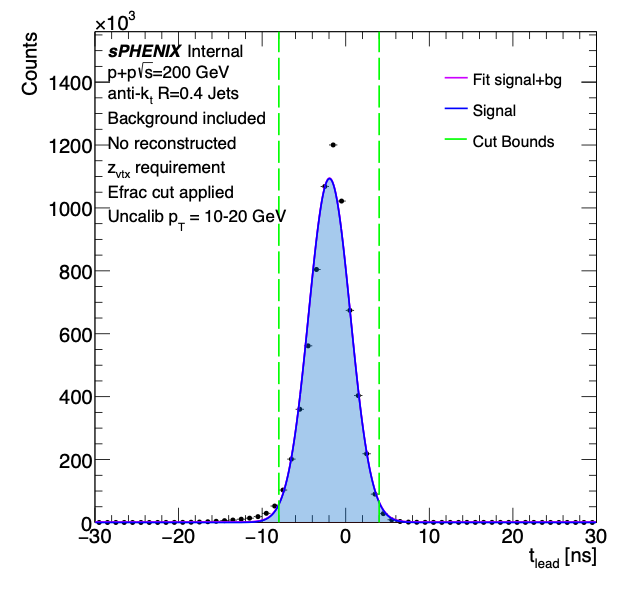
\includegraphics[width=0.48\linewidth]{Figures/jet_bkg_cuts/lead_jet_time_cut.png}
    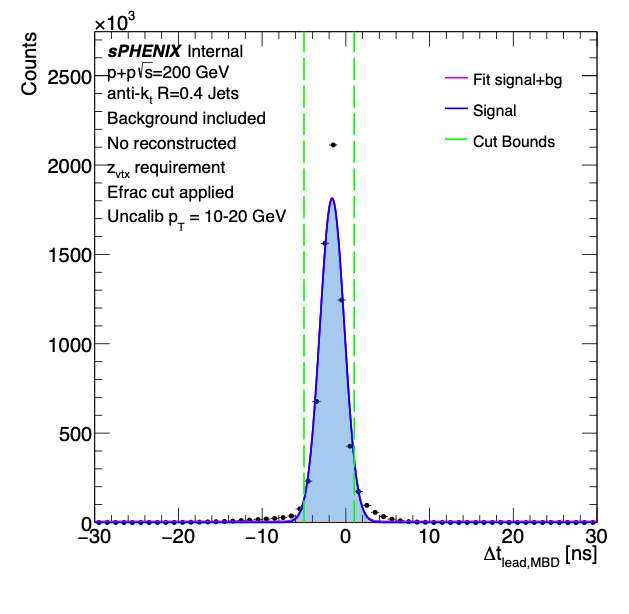
\includegraphics[width=0.48\linewidth]{Figures/jet_bkg_cuts/lead_jet_mbd_time_cut.png}
    \caption{Leading jet time (left) and leading jet--MBD time (right) distributions for events passing the energy fraction jet background cuts for example uncalibrated leading jet $p_{T}$ range of 10--20~GeV. Extracted signal and signal + background distributions are shown within the cut window. Efficiencies are extracted from these signal and signal + background distributions.}
    \label{fig:lead_jet_time_mbd_time_cut}
\end{figure}

\begin{figure}
    \centering
    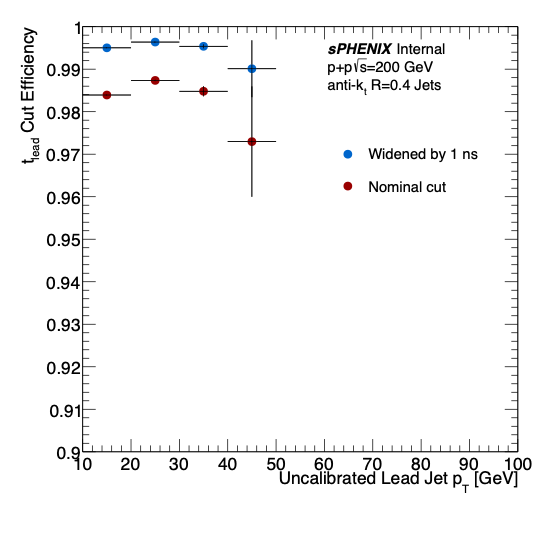
\includegraphics[width=0.48\linewidth]{Figures/jet_bkg_cuts/lead_time_cut_efficiency.png}
    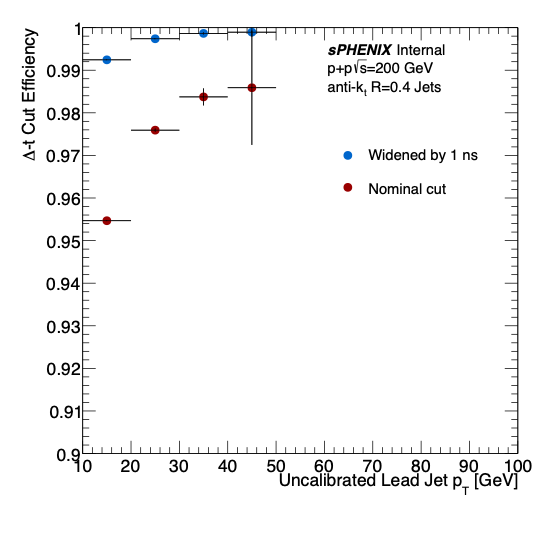
\includegraphics[width=0.48\linewidth]{Figures/jet_bkg_cuts/deltat_cut_efficiency.png}
    \caption{Timing cut efficiencies as a function of leading jet $p_{T}$ for the energy fraction jet background cut and the leading jet time + jet--MBD time cut.}
    \label{fig:timing_cut_efficiencies}
\end{figure}

\begin{figure}
    \centering
    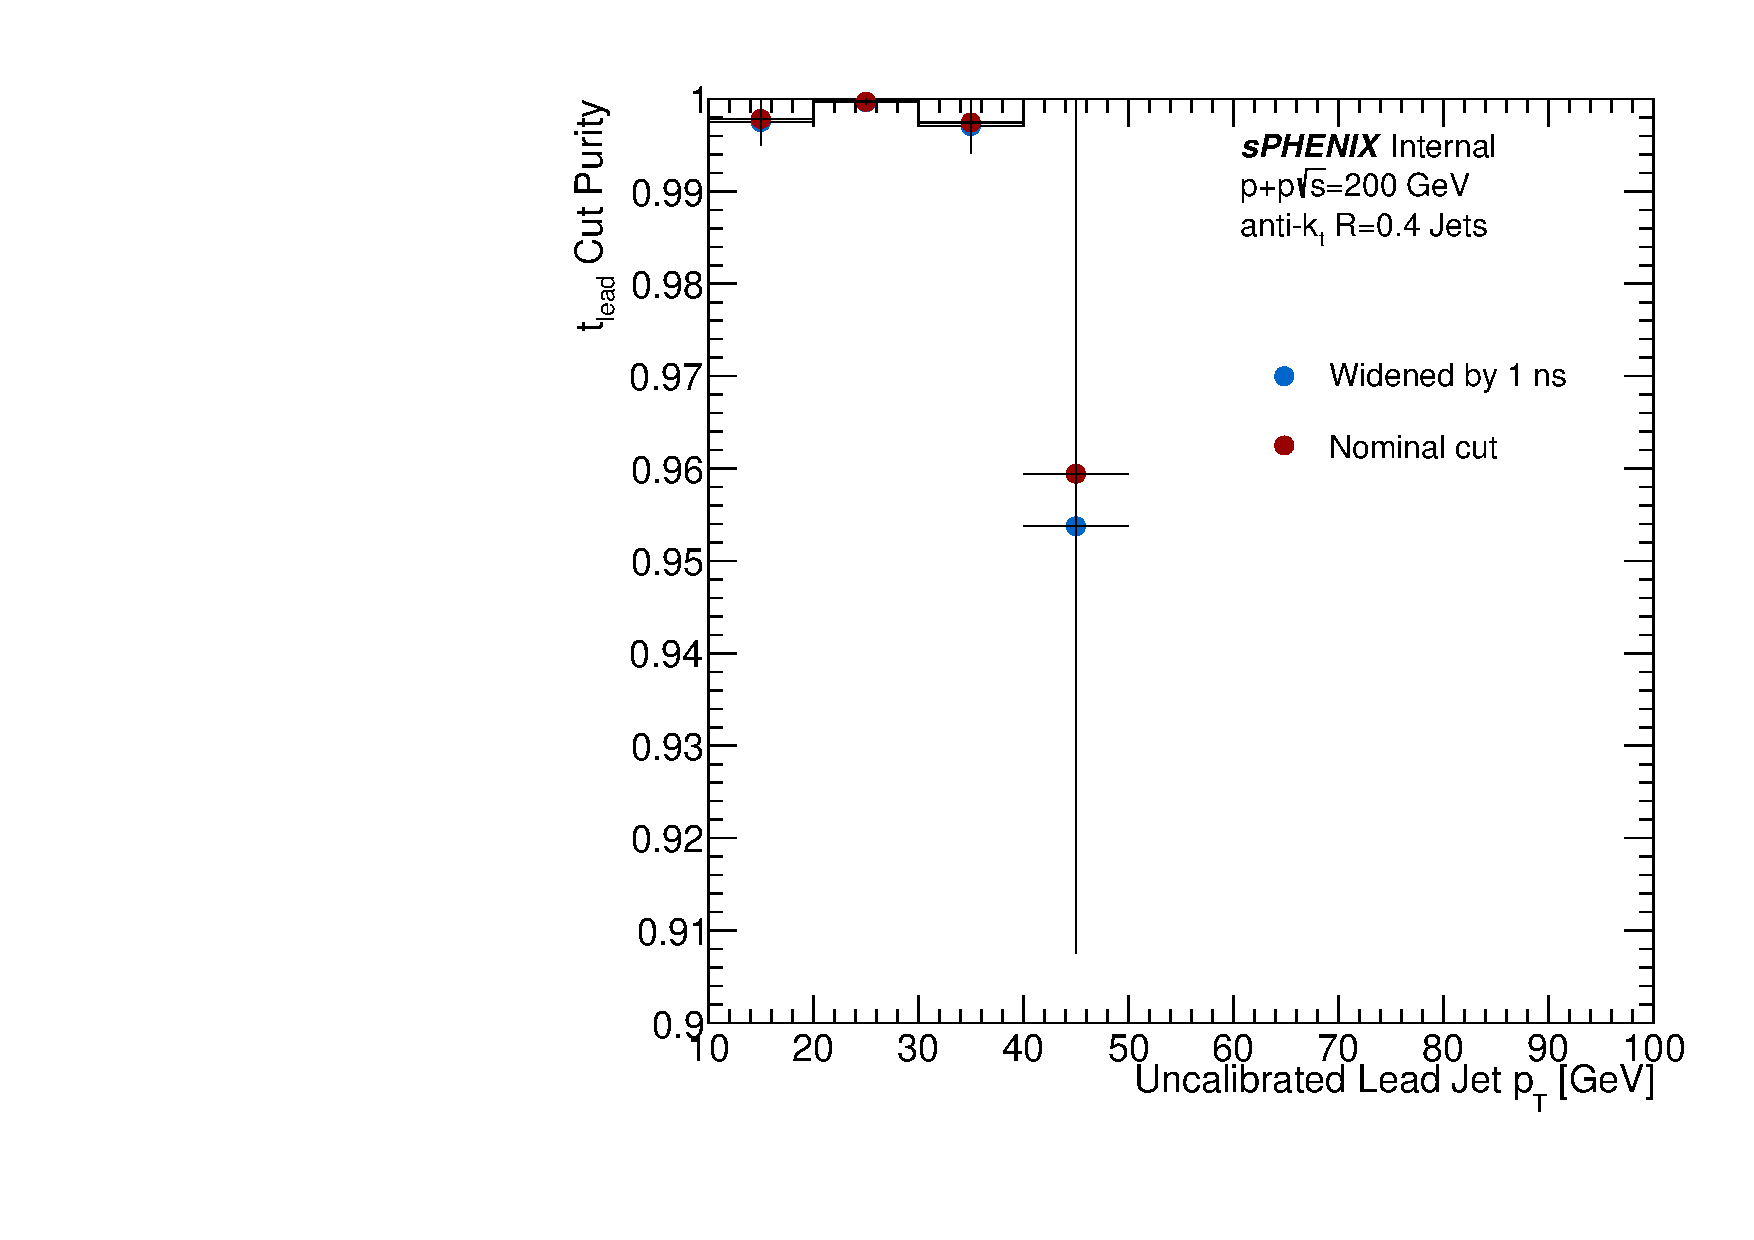
\includegraphics[width=0.48\linewidth]{Figures/jet_bkg_cuts/lead_time_cut_purity.pdf}
    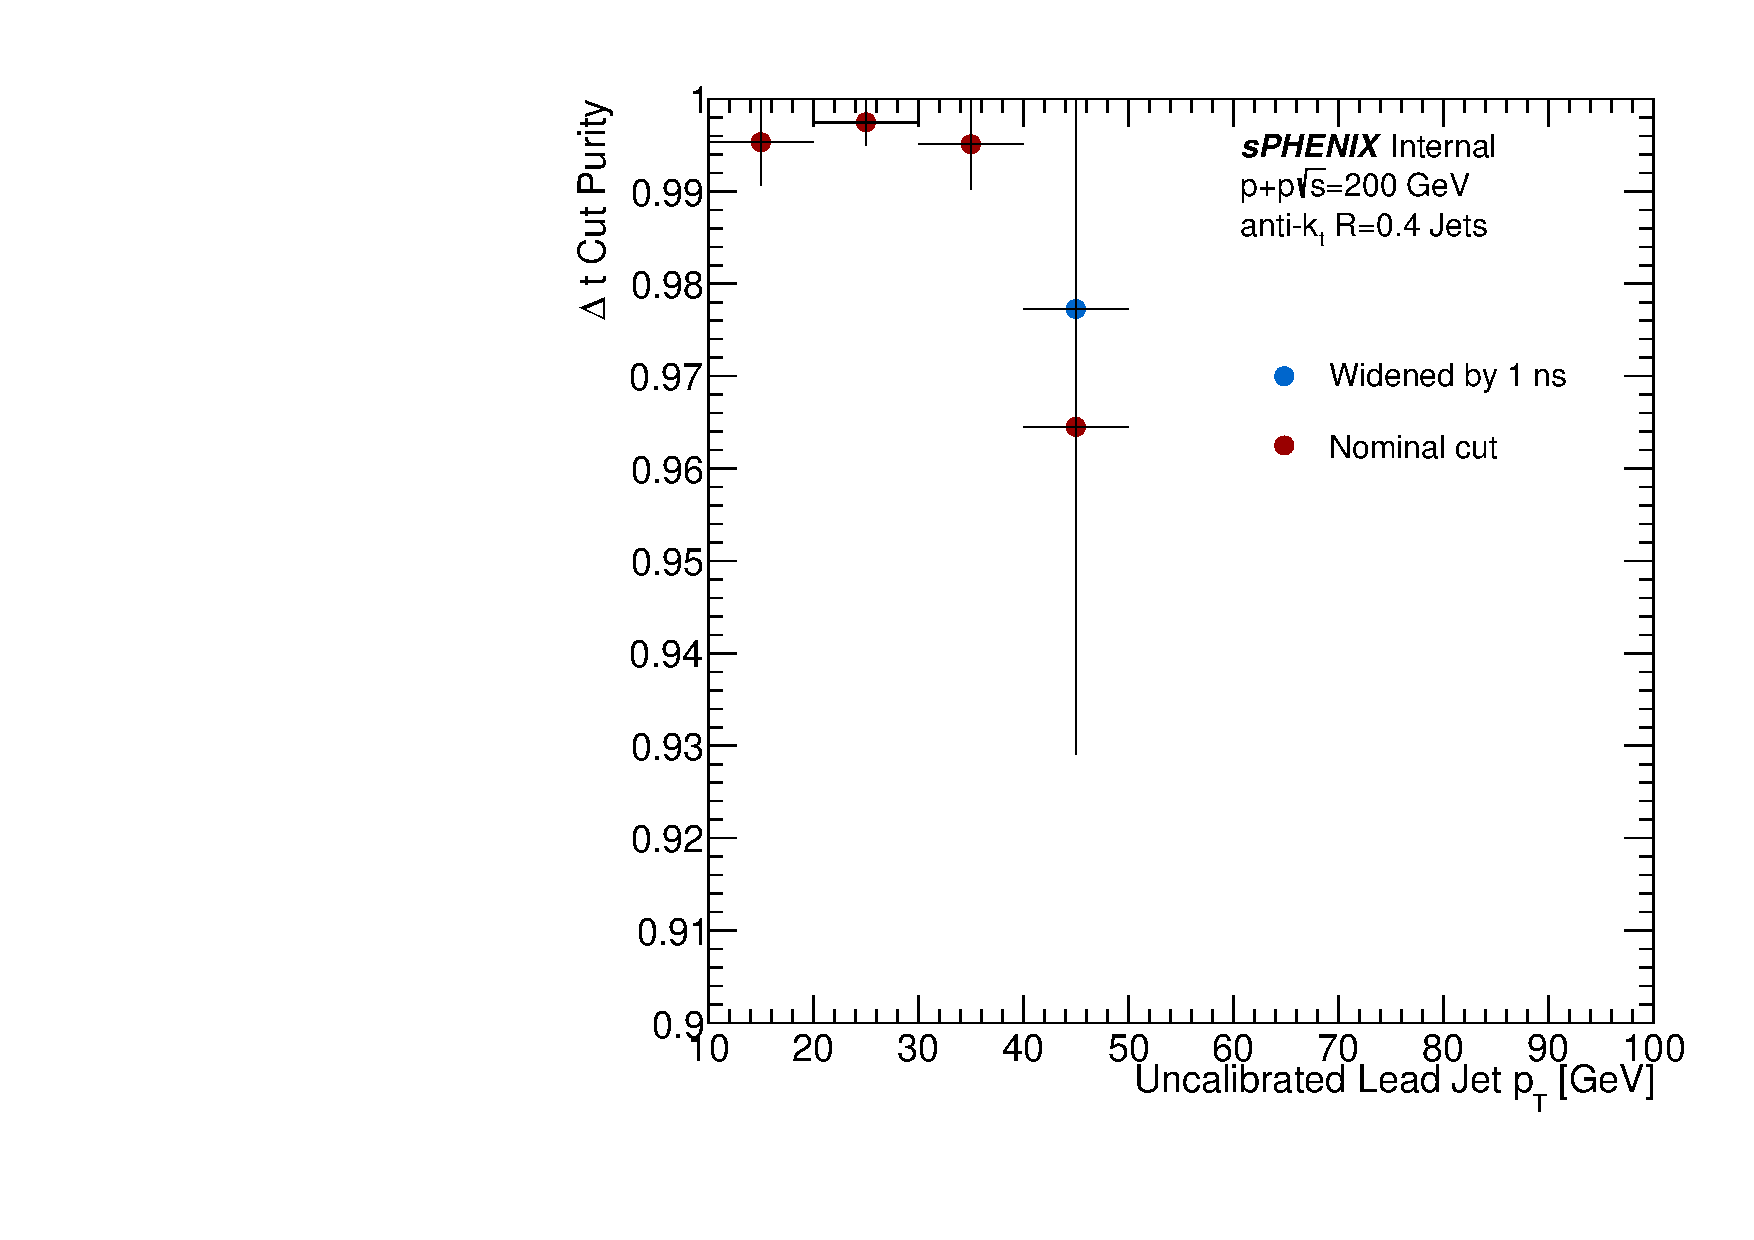
\includegraphics[width=0.48\linewidth]{Figures/jet_bkg_cuts/deltat_cut_purity.pdf}
    \caption{Timing cut purity as a function of leading jet $p_{T}$ for the energy fraction jet background cut and the leading jet time + jet--MBD time cut.}
    \label{fig:timing_cut_purity}
\end{figure}

